	\subsection{Fundamentals about signal processsing}
	\subsubsection{Definition of a signal}
	Lopez's PhD \cite{lopez} gives a good presentation of the state of the art.
	Many notations and definitions are kept from this PhD.

	\begin{thdef}\label{sig} (Signal)
		Generally, a signal is a temporal variable, which takes a value from $\mathbb{R}$ at each time t.
		We denote $x(t)$ the value of the signal $x$ at the instant $t$.
		When dealing with discrete time events, the time will be represented by $k$.
		Then we denote about $x(k)$, which is said to be a sample.
		$\{x(k)\}_{k \geq 0}$ denotes all the values possible for the signal x.
		In the rest of this report, we will discuss about vectors of signals $\textbf{x}$, where $\textbf{x}(k) \in \mathbb{R}^{n}$
	\end{thdef}

	\subsubsection{Linear Time Invariant Filters (LTI filters)}
	A filter, denoted by its transfer function $\mathcal{H}$, is an application which transforms a signal vector $\boldsymbol{u}$ (with $dim(\boldsymbol{u}) = n_u$ )
	into a signal $\boldsymbol{y} = \mathcal{H}(\boldsymbol{u})$, of size $dim(\boldsymbol{y}) = n_y$ . When $n_u = n_y = 1$, we speak about Single Input Single Output
	(SISO) filters. In other cases, we speak about Multiple Input Multiple Output (MIMO) filters.

	\begin{thdef} (Linear Time Invariant Filter)
		Linearity:
		$$ \mathcal{H}(\alpha \cdot \boldsymbol{u}_1+ \beta \cdot \boldsymbol{u}_2)= \alpha\cdot\mathcal{H}(\boldsymbol{u}_1) +  \beta\cdot\mathcal{H}(\boldsymbol{u}_2)$$

		Time invariance:
		$$ \{\mathcal{H}(\boldsymbol{u})(k-k_0)\}_{k\geq0} = \mathcal{H}(\{\boldsymbol{u}(k-k_0)\}_{k \geq 0} ) $$
	\end{thdef}

	\subsubsection{Impulse response}
	\begin{thdef} (Impulse Response)
	A SISO filter may be defined by its impulse response, denoted $h$. $h$ is the
	impulse response of H to the impulsion of Dirac.
	Indeed each input can be described as a sum of Dirac impulsions:
	$$u=\sum_{i\geq0}u(l)\delta_l$$
	where $\delta_l$ is a Dirac impulsion centered in $l$, that is:
	\begin{equation}
		\delta(k) =
		\begin{cases}
			1 & \hspace{5pt} when \hspace{5pt} k=l\\
			0 & \hspace{5pt} else\\
		\end{cases}
	\end{equation}
	The linearity condition of $\mathcal{H}$ implies: $\mathcal{H}(u) = \sum_{l\geq0}u(l)\mathcal{H}(\delta_l)$.
	Time invariance gives: $\mathcal{H}(\delta_l)(k)=h(k-l)$.
	Then the computation from inputs to outputs takes this form:
	$$y(k)=\sum_{l\geq0}u(l)h(k-l)=\sum_{l=0}^ku(k)h(k-l)$$
	This corresponds with the convolution product definition of $u$ by $h$, denoted $y = h * u$.
	%Dealing with MIMO filters, we have $\boldsymbol{h} \in \mathbb{R}^{n_y \times n_u}$ as the impulse response of $\mathcal{H}$. $\boldsymbol{h}_{i,j}$ is the response on the
	Dealing with MIMO filters, we have $\boldsymbol{h} \in \mathbb{R}^{n_y \times n_u}$ as the impulse response of $\mathcal{H}$. $\boldsymbol{h}_{i,j}$ is the response on the
	ith output to the Dirac implusion on the j-th input.
	The precedent equation becomes:
	$$y_i(k)=\sum_{j=1}^{n_u}\sum_{l\geq}^lu_j(l)h_{i,j}(k-l), \hspace{5pt} \forall 1 \leq i \leq n_y$$
	
	\end{thdef} 

	\subsubsection{Worst-Case Peak Gain (WCPG) of a Filter: the maximum amplification expectable}
	\begin{thdef} (Worst-Case Peak Gain)
		The worst case peak gain is defined as the maximum amplification
		possible over all potential inputs through the filter.
		$$\|\mathcal{H}\|_{wcpg}=\sup_{u\neq0}\frac{\|h*u\|_{l^{\infty}}}{\|u\|_{l^{\infty}}}$$
		with $h$ the impulse response of $\mathcal{H}$, $u$ the input signal, and $h * u$ the convolution product of $h$ by $u$ (output of the
				filter).
	
	\end{thdef}

	\subsection{FIR and IIR: two filters families}
	There is two types of LTI filters: \textit{Finite impulse response} (FIR) and \textit{Infinite impulse response} (IIR) filters.
	Formally, we define the impulse response as finite when:
	\begin{equation} \label{finimp}
		\exists n \in \mathbb{N} | \forall k \geq n, h(k)=0
	\end{equation}
	The smallest $n$ verifying \ref{finimp} is referred as the order of the filter. So a n-order FIR can be described by the
	following equation:
	\begin{equation} \label{firdef}
		y(k)=\sum_{i=0}^n b_i u(k-i)
	\end{equation}

	An IIR will be described as following:
	\begin{equation} \label{iirdef}
		y(k)=\sum_{i=0}^n b_i u(k-i) - \sum_{i=0}^n a_i y(k-i)
	\end{equation}

	Here one can observe that the output at time $k$ depends also on all previous $n$ outputs (loopback). One can
	also see that a FIR can be seen as an IIR with $\forall i \in [0,n],a_i=0$
	The impulse response can then be deduced from \ref{iirdef} by resolving the recurrence relation:

	\begin{equation}
		h(k) =
		\begin{cases}
			0 & \hspace{5pt} when k<l\\
			b_k - \sum_{l=1}^n a_l h(k-l) & \hspace{5pt} when 0\leq k \leq n\\
			\sum_{l=1}^n a_l h(k-l) & \hspace{5pt} when n< k\\
		\end{cases}
	\end{equation}

	\subsection{Different realizations: how to compute the output of a filter?}
	\begin{thdef} (realization)
	A realization can be defined as an algorithm describing how to compute outputs
	from inputs. However, a realization does not describes the details of basic operations (format, size, order,
	rounding, etc...)
	\end{thdef}
	It is important to know that all realizations of a filter are mathematically equivalent to each other (infinite
	precision). But in finite precision, rounding aspects have a huge impact on the correctness of results.
	Most of the time in this report, we will describe realizations as forms.

	\subsubsection{Direct and transposed forms}
	Direct and transposed forms are classic realizations. A good description of these forms can be found in Lopez’ and Hilaire’s PhDs \cite{lopez} \cite{hilaire}. 
	The direct form has been implemented and in the FoPoCo project,
	you can see the hardware implementation an IIR on figure \ref{iirpic}

\begin{figure*} \label{iirpic}
  \centering
  \begin{tikzpicture}
     \draw[dotted,black, fill=yellow!20] (-5ex,-3.5ex) rectangle +(69ex,-15ex);   
     \node[black]  at (-2ex,-17.5ex) {{\small SOPC}};   
    \draw[hwbus] (-8, 0) node[left] {$u(k)$} --  ++(8, 0)  ;
    \draw[hwbus,->] (-8, 0) --  ++(3, 0); % just for the arrow
    \foreach \i in {0,...,3} {
      \draw[hwbus, ->] ($(8*\i, 0)$) --  ++(0, -5);
      \draw[hwblock] ($(8*\i, -5)$) -- ++(3, 0) -- ++(-3, -4) -- ++(-3, 4) -- cycle; 
      \node (n) at ($(8*\i , -6.5)$)  {$b_{\i}$} ;
%      \draw ($(8*\i  + 0.5, -11)$) node[left,tt=black!50] {\footnotesize $p_b(k,\i)$} ;
%      \draw ($(8*\i  - 0.2, -11)$) node[right,text=black!50] {\footnotesize $p_b(k,\i)$} ;

%      \draw[hwbus, ->] ($(8*\i ex, 0ex)$) --  ++(0, -5ex);
    }

    
    \draw[hwbus] (0, -9) -- ++(0,-6);
      \coordinate (n) at  (0,-15);
    \foreach \i in {1,...,3} {
      \draw[line width=3pt] ($(8*\i  - 4, -3)$) --  +(0, 6);
      \draw[hwbus] ($(8*\i  - 8, 0)$) --  +(8,0) node [above,text=blue] {\footnotesize $u(k-\i)$};
      \draw[hwbus,->] ($(8*\i  - 8, 0)$) --  ++(3, 0); % just for the arrow
      % The adders 
      \coordinate (nm1) at  (n.east);
      \draw ($(8*\i , -15)$) node[hwblock,circle,minimum height=3] (n) {$+$};
      \draw[hwbus, ->]  ($(8*\i , -9)$) -- (n.north);
      \draw[hwbus, ->]  (nm1) -- (n.west);
      \draw[hwbus]  (n.east) -- ++ (3,0);
    }

    \draw (74, -15) node[hwblock,align=center] (fr) {final\\round} ;
    \draw[hwbus, <-] (fr.west) -- ++(-15,0) node [near end] {/} node [near end,below] {\footnotesize$(\msbout, p-g$)} node[near start,above] {$\appr{y}(k)$} -- ++(-1,0) ;
    \draw[hwbus, ->] (fr.east) -- ++(8,0) node [midway] {/} node [midway,below] {\footnotesize$(\msbout,p)$} node[right] {$\yout(k)$} ;

    \foreach \i in {1,...,3} {
      \draw[hwbus, ->] ($(-8*\i  + 60 , 0)$) --  ++(0, -5);
      \draw[hwblock] ($(-8*\i  + 60 , -5)$) -- ++(3, 0) -- ++(-3, -4) -- ++(-3, 4) -- cycle; 
      \node (ai) at ($(-8*\i  + 60 , -6.5)$)  {$a_{\i}$} ;
      %\draw ($(-8*\i  +60 + 0.5, -11)$) node[left,text=black!50] {\footnotesize $p_a(k,\i)$} ;
      %\draw ($(-8*\i  +60 - 0.2, -11)$) node[right,text=black!50] {\footnotesize $p_a(k,\i)$} ;
      \draw ($(-8*\i  + 60 , -15)$) node[hwblock,circle,minimum height=3] (n) {$+$};
      \draw (n.north) node[left]{\bf -};
      \draw[hwbus, ->] ($(-8*\i  + 60, -9)$) --  (n.north);
      \draw[hwbus, <-] (n.west) -- ++(-5,0);
      % The registers
      \draw[hwbus] ($(-8*\i  + 60  +8, 0)$) --  ++(-8, 0) node [above,text=blue] {\footnotesize $\appr{y}(k-\i)$};
      \draw[hwbus,->] ($(-8*\i  + 60  +8, 0)$) --  ++(-3, 0); % just for the arrow
      \draw[line width=3pt] ($(-8*\i  +60 + 4, -3)$) --  +(0, 6);
    }
    \draw[hwbus] ($(60 , 0)$) --  ++(0,-15);
    \draw[hwbus,<-] ($(60 , -5)$) --  ++(0,-5);


  \end{tikzpicture}

\caption{Abstract architecture for the direct form realization of an LTI filter \label{fig:ltiarch}}
\end{figure*}

	\subsubsection{State-space representation: a recurrence to define an infinite response}
	This type of realization consists in expressing the evolution of a system considering it’s state at time k. In
	continuous time, it is described by differential equations at first order. In discret time (in which we
	are interested in), it is described by a simple recurrence:
	\begin{equation} \label{abcddef}
		\begin{cases}
			\boldsymbol{x}(k+1)= \boldsymbol{Ax}(k) + \boldsymbol{Bu}(k) \\
			\boldsymbol{y}(k+1)= \boldsymbol{Cx}(k) + \boldsymbol{Du}(k)
		\end{cases}
	\end{equation}

	Where $\boldsymbol{x}(k) \in \mathbb{R}^{n_x}$ is the state vector,
	$\boldsymbol{u}(k) \in \mathbb{R}^{n_u}$ is the input vector and
	$\boldsymbol{y}(k) \in \mathbb{R}^{n_y}$ is the output vector, at time k.
	The matrices $\boldsymbol{A} \in \mathbb{R}^{n_x \times n_x}$ , $\boldsymbol{B} \in \mathbb{R}^{n_x \times n_u}$,
	$\boldsymbol{C} \in \mathbb{R}^{n_y \times n_x}$, and $\boldsymbol{D} \in \mathbb{R}^{n_y \times n_u}$,
	with $\boldsymbol{x}(0)$ are sufficient to describe an LTI filter, with convention $\boldsymbol{x}(k)=\boldsymbol{u}(k)=0 \hspace{5pt} | \hspace{5pt} \forall k<0$.

	\subsection{The Specialized Implicit Form (SIF): a unified representation}
	\subsubsection{Definition}
	The specialized implicit form (SIF) was introduced in \cite{sifd} and is well detailed in Hilaire's PhD and associated papers \cite{hilaire,sif}. 
	The classical state-space representation is intuitive,
	but it doesn't takes into account the reality of implementation.
	Indeed, dealing with finite precision and error amplification, the order in which operations are done becomes crucial.
	Another idea is to have a unique representation for any realization of LTI filters,
	that allows to compute every degradation measures instead of redevelopping them for each new realization.
	This form distinguishes computations done at one time from computations done the other times. As well as
	in a state-space, we have $\boldsymbol{x}_i$ as state variables, but in addition to that, $\boldsymbol{t}_i$ are intermediate variables.
	The SIF is described as following:
	\begin{equation} \label{sifdef}
		\begin{pmatrix}
			\boldsymbol{J} & \boldsymbol{0} & \boldsymbol{0} \\
			\boldsymbol{-K} & \boldsymbol{I}_{n_x} & \boldsymbol{0} \\
			\boldsymbol{-L} & \boldsymbol{0} & \boldsymbol{I}_{n_y} 
		\end{pmatrix}
		\begin{pmatrix}
			\boldsymbol{t} (k+1)  \\
			\boldsymbol{x} (k+1)  \\
			\boldsymbol{y} (k) 
		\end{pmatrix}
		=
		\begin{pmatrix}
			\boldsymbol{0} & \boldsymbol{M} & \boldsymbol{N} \\
			\boldsymbol{0} & \boldsymbol{P} & \boldsymbol{Q} \\
			\boldsymbol{0} & \boldsymbol{R} & \boldsymbol{S} 
		\end{pmatrix}
		\begin{pmatrix}
			\boldsymbol{t} (k)  \\
			\boldsymbol{x} (k)  \\
			\boldsymbol{u} (k) 
		\end{pmatrix}
	\end{equation}
	With $n_t$, $n_x$, $n_y$ and $n_u$ the sizes of $\boldsymbol{t}$,$\boldsymbol{x}$,$\boldsymbol{y}$ and $\boldsymbol{u}$, respectively.
	$\boldsymbol{J}$, is a lower triangular matrix, with
	diagonal entries equal to 1. Then we have the following dimensions for the previous matrices:

	\begin{eqnarray}
		\boldsymbol{J} \in \mathbb{R}^{n_t \times n_t},\boldsymbol{M} \in \mathbb{R}^{n_t \times n_x},\boldsymbol{N} \in \mathbb{R}^{n_t \times n_u}, \nonumber \\
		\boldsymbol{K} \in \mathbb{R}^{n_x \times n_t},\boldsymbol{P} \in \mathbb{R}^{n_x \times n_x},\boldsymbol{Q} \in \mathbb{R}^{n_x \times n_u}, \\
		\boldsymbol{L} \in \mathbb{R}^{n_y \times n_t},\boldsymbol{R} \in \mathbb{R}^{n_y \times n_x},\boldsymbol{S} \in \mathbb{R}^{n_y \times n_u}, \nonumber \\
	\end{eqnarray}

	The best way to understand the SIF may be to see it as an algorithm, each line of the equation \ref{sifdef} corresponding to a sequential step of the computation.
	The algorithm results as follows:
	\begin{algorithm}
		\For{int i = 0 ; $i \leq n_t$; i++}{
			$\boldsymbol{t}_i(k+1) \leftarrow - \sum_{j<i} \boldsymbol{J}_{ij}\boldsymbol{t}_j(k+1) + \sum_{j=1}^{n_x} \boldsymbol{M}_{ij}\boldsymbol{x}_j(k) + \sum_{j=1}^{n_u} \boldsymbol{N}_{ij}\boldsymbol{u}_j(k)$
		}
		\For{int i = 0 ; $i \leq n_x$; i++}{
			$\boldsymbol{x}_i(k+1) \leftarrow - \sum_{j=1}^{n_t} \boldsymbol{K}_{ij}\boldsymbol{t}_j(k+1) + \sum_{j=1}^{n_x} \boldsymbol{P}_{ij}\boldsymbol{x}_j(k) + \sum_{j=1}^{n_u} \boldsymbol{Q}_{ij}\boldsymbol{u}_j(k)$
		}
		\For{int i = 0 ; $i \leq ny$; i++}{
			$\boldsymbol{y}_i(k+1) \leftarrow - \sum_{j=1}^{n_t} \boldsymbol{L}_{ij}\boldsymbol{t}_j(k+1) + \sum_{j=1}^{n_x} \boldsymbol{R}_{ij}\boldsymbol{x}_j(k) + \sum_{j=1}^{n_u} \boldsymbol{S}_{ij}\boldsymbol{u}_j(k)$
		}
		\caption{Computation of SIF outputs from inputs}
	\end{algorithm}

	Here, it is important to see that the form of $\boldsymbol{J}$ allows to compute the $\boldsymbol{t}_i$ sequentially. The algorithm can
	then be described as follows:
	\begin{algorithm} \label{algomat}
		\For{int i = 0 ; $i \leq n_t$; i++}{
			$\boldsymbol{t}_i(k+1) \leftarrow - \boldsymbol{J'}_{i}\boldsymbol{t}(k+1) + \boldsymbol{M}_{i}\boldsymbol{x}(k) +\boldsymbol{N}_{i}\boldsymbol{u}(k)$
		}
		\For{int i = 0 ; $i \leq n_x$; i++}{
			$\boldsymbol{x}_i(k+1) \leftarrow - \boldsymbol{K}_{i}\boldsymbol{t}(k+1) + \boldsymbol{P}_{i}\boldsymbol{x}(k) +\boldsymbol{Q}_{i}\boldsymbol{u}(k)$
		}
		\For{int i = 0 ; $i \leq ny$; i++}{
			$\boldsymbol{y}_i(k+1) \leftarrow - \boldsymbol{L}_{i}\boldsymbol{t}(k+1) + \boldsymbol{R}_{i}\boldsymbol{x}(k) + \boldsymbol{S}_{i}\boldsymbol{u}(k)$
		}
		\caption{Simplified matricial algorithm}
	\end{algorithm}

	With $\boldsymbol{J'} = \boldsymbol{J} - I_{n_t}$.

	Values of the vector $\boldsymbol{t}(k+1)$ are computed and used at the same iterations, so they are not kept in memory.
	As the equation is mostly full of zeros, it is more convenient to use it’s compressed formulation, wich is denoted
	as the $\boldsymbol{Z}$:
	
	\begin{equation} \label{zmatrix}
		\boldsymbol{Z}=
		\begin{pmatrix}
			\boldsymbol{-J} & \boldsymbol{M} & \boldsymbol{N} \\
			\boldsymbol{K} & \boldsymbol{P} & \boldsymbol{Q} \\
			\boldsymbol{L} & \boldsymbol{R} & \boldsymbol{S} 
		\end{pmatrix}
	\end{equation}
	The community usually takes $-\boldsymbol{J}$ for simplicity within further computations.

	We can of course bind the SIF with the ABCD (classic state-space) form, which gives:

	\begin{eqnarray} \label{abcdtranspose}
		\boldsymbol{A_Z} = \boldsymbol{KJ}^{-1}\boldsymbol{M} +\boldsymbol{P}, \hspace{5pt}
		\boldsymbol{B_Z} = \boldsymbol{KJ}^{-1}\boldsymbol{N} +\boldsymbol{Q}, \nonumber \\
		\boldsymbol{C_Z} = \boldsymbol{LJ}^{-1}\boldsymbol{M} +\boldsymbol{R}, \hspace{5pt}
		\boldsymbol{D_Z} = \boldsymbol{LJ}^{-1}\boldsymbol{N} +\boldsymbol{S}, \nonumber \\
	\end{eqnarray}

	With:
	\begin{eqnarray}
		\boldsymbol{A_Z} \in \mathbb{R}^{n_x \times n_x},
		\boldsymbol{B_Z} \in \mathbb{R}^{n_x \times n_u}, \nonumber \\
		\boldsymbol{C_Z} \in \mathbb{R}^{n_y \times n_x},
		\boldsymbol{D_Z} \in \mathbb{R}^{n_x \times n_u},
	\end{eqnarray}

	\subsubsection{Optimal SIF realization}
		Here, we won't discuss the optimality of the SIF description.
		This optimality is up to the user, who may have a lot of good reasons not to design a realization that seem optimal for us.
		The optimization of the realization is a job done at LIP6 in the PEQUAN team, under the metalibm ANR project.
		The present work is just a hardware backend for the optimization part.
		The expected use of this work is shown on figure \ref{fig:workflow}.


		\begin{figure}[h] 
		  \centering
		  \begin{tikzpicture}[x=1cm,y=1cm]
			\draw (-9.5, 1.0) -- (-8,1.0) [->, thick] node[above,near start, text width = 3cm, align=center]{User filter specification};
			\draw (-3.5, 1.0) -- (0.0,1.0) [->, thick] node[below,xshift=-1.8cm]{$\begin{pmatrix}\boldsymbol{-J} & \boldsymbol{M} & \boldsymbol{M}_t \\ \boldsymbol{K} & \boldsymbol{P} & \boldsymbol{M}_x \\ \boldsymbol{L} & \boldsymbol{R} & \boldsymbol{M}_y \end{pmatrix}$};
			\draw (-8,0.0) rectangle ++(4.5,2)[thick] node [midway, text width = 4cm, align=center]{Relization Optimization \\ by \\ Hilaire, Volkova  \\ team PEQUAN, LIP6}; 
			\draw (0.0,0.0) rectangle ++(3.0,2)[thick] node [midway, text width = 3cm, align=center]{Flopoco core generation \\ (this work)}; 

			\draw (4,0) rectangle ++(2.5,2)[thick] node [midway]{VHDL}; 
			\draw (3.0, 1) -- (4,1) [->, thick] node[above,near start]{};

		  \end{tikzpicture}

		\caption{Workflow overview of tools usage \label{fig:workflow}}
		\end{figure}


	\subsection{Implementation: what can be done in practise?}

	\subsubsection{The FloPoCo Framework: computing just right}
		FloPoCo is a C++ framework \cite{DinechinPasca2011-DaT} which first purpose is to generate floating point cores in VHDL.
		Although it may have some pertinence in the ASIC design market, it main target is the configuration of FPGAs as computing units.
		Indeed, FPGAs are a rising market for embedded computing, because they offer full reconfigurability and a relatively good balance between computation power and price.

		More information is available at \url{http://flopoco.gforge.inria.fr/}

	In this work, we propose to implements SIFs using the SOPCs arithmetical core from FloPoCo.
	SOPC stands for Sum of Producs by Constants, and is a KCM-multiplier based architecture.
	The details of the SOPC architecture has been described in \cite{sums}.

	\subsubsection{KCM multipliers: an architecture to efficiently compute products on FPGAs}
	To be quick, a KCM multiplier is designed to fully use the power of look-up tables (LUTs) in an FPGA.
	To do so, it partitions the constant into chunks which match the size of a LUT.
	Then, tabulating the multiplications, we end up with a final sum to compute the product.
	This has been first described by K.Chapman in \cite{Chapman93:edn}.
	The detail of implementation is visible on figure \ref{fig:FixRealKCM}

\begin{figure}[b]
  \begin{center}
  \begin{tikzpicture}
    \footnotesize 
    \node at (-1em,0)  {$x_i=$} ;
    \foreach \x in {1,...,18} {
%    \draw[] ($(-5*\x ex, -7ex)$) -- ($(-5*\x ex, -5ex)$) node[above] {$2^\x$} ;
      \node (n) at ($(3.4*\x ex, 0ex)$)  {$b_{\x}$} ;
      \draw[black!25, very thin] ($(n)+(1.7ex,1.5ex)$) -- ++(0, -3ex);
    }
    \node[draw, thick, rectangle, minimum width = 3.4*6ex, minimum height=3ex] (d1) at (3.4*3ex+1.7ex,0) {} ;
    \node[hwblock, minimum width=20ex,minimum height=6ex] (T1) at ($(d1)+(0,-10ex)$) { $T_{i1}: \circ_p(c_i\times d_{i1})$};
    \draw[hwbus,->] (d1.south) --  (T1.north) node[midway,right] {$d_{i1}$};

    \node[draw, thick, rectangle, minimum width = 3.4*6ex, minimum height=3ex] (d2) at (3.4*9ex+1.7ex,0) {} ;
    \node[hwblock, minimum width=15ex] (T2) at ($(d2)+(0,-10ex)$) { $T_{i2}$};
    \draw[hwbus,->] (d2.south) --  (T2.north) node[midway,right] {$d_{i2}$};

    \node[draw, thick, rectangle, minimum width = 3.4*6ex, minimum height=3ex] (d3) at (3.4*15ex+1.7ex,0) {} ;
    \node[hwblock, minimum width=10ex,minimum height=3.5ex] (T3) at ($(d3)+(0,-10ex)$) { $T_{i3}$};
    \draw[hwbus,->] (d3.south) --  (T3.north) node[midway,right] {$d_{i3}$};

    
    \node[hwblock, minimum width=50ex] (sum) at ($(T2)+(0,-11.3ex)$) {\Large $+$};
    \draw[hwbus,->]  (T1.south) --  ($(sum.80)!(T1)!(sum.north)$) % This means: point that is the projection of T1 on the line  (sum.80) -- (sum.north)
       node[near start] {$/$} node[near start,left] {$q_i+g$}          node[near end,right] {$\widetilde{t}_{i1}$};
    \draw[hwbus,->]  (T2.south) --  ($(sum.80)!(T2)!(sum.north)$) node[near start] {$/$} node[near start,left] {$q_i-\alpha+g$}   node[near end,right] {$\widetilde{t}_{i2}$};
    \draw[hwbus,->]  (T3.south) -- ($(sum.80)!(T3)!(sum.north)$) node[near start] {$/$} node[near start,left] {$q_i-2\alpha+g$}  node[near end,right] {$\widetilde{t}_{i3}$};

    \draw[hwbus,->] (sum.south) --  ++(0,-6ex) node[near start] {$/$} node[near start,left] {$q_i+g$} node[near end,right] {$\widetilde{p}_i\approx c_ix_i$};
 \end{tikzpicture}
\end{center}
\caption{The FixRealKCM method when $x_i$ is split in 3 chunks   \label{fig:FixRealKCM}}
\end{figure}

	\subsubsection{SOPCs: exploiting full parallel architecures}

	The SOPC architecture keeps the same idea.
	The difference is, the summation architecture is mutualized through the $n_c$ products in a bit-heap based architecture implemented by flopoco.
	The detail is visible on figure \ref{fig:Overall architecture}.

\begin{figure}
  \begin{center}
  \begin{tikzpicture}
    \footnotesize 
    
    \node[hwblock, align=center,minimum width=60ex] (sum) at ($(32ex,-5ex)$) {Bit-heap based \\ summation architecture};

    \foreach \i in {0,...,3} {
      \node (x) at  ($(15*\i ex+10ex, 17ex)$) {$x_\i$};
      \coordinate (xb) at  ($(x)+(0, -3ex)$);
      \draw[hwbus,very thick] (x) --  (xb);
      
      \foreach \k in {1,...,3} {
        \node[hwblock, minimum width=5ex] (T) at ($(15*\i ex+4.5*\k ex,7ex-1*\k ex)$) { $T_{\i\k}$};
        \draw[hwbus,thick,<-]  (T.north) -- ++(0,+4ex) node [midway] {/}node [midway,right] {$\alpha$} -- (xb);
        \draw[hwbus,->] (T.south) --  ($(sum.north)!(T)!(sum.80)$);
      }
    }

    \draw[hwbus,->] (sum.south) --  ++(0,-6ex) node[near start] {$/$} node[near start,left] {$p$} node[near end,right] {$y$};
 \end{tikzpicture}
\end{center}
\caption{KCM-based SPOC architecture for $n_c=4$, each input being split into 3 chunks  \label{fig:Overall architecture}}
\end{figure}

	\subsubsection{Precision concerns}

	In SOPCs architectures, the accuracy is deducible from the inputs/outputs specifications and the size of the constants.

	This is described in \cite{sums}.

	Dealing with feedback inputs, the question of precision is more complicated.
	Indeed, when results loop back to inputs, as soon as we are in finite precision, the error is amplified by a certain amount, depending on the coefficients, at each pass through the filter.

	In this case the solution in the industry is to build an equivalent FIR filter by resolving the recurrence.
	This leads to build an accurate hardware, but at the price of a huge waste of logic.
	The present work is an answer to this problem, trying to compute just right, keeping the recurrence and saving hardware.

	The main idea to dimension such filters is to consider the total error as a single filter.
	The result of this filter is then added to the perfect filter to get the final output.

	In finite precision, sizes are constrained to be all the same. The demonstration of the size computation has been described in Lopez' PhD \cite{lopez}.
	The idea now is to see what we can do in arbitrary precision, trying to save a maximum of logic while keeping a right result on the precision required by the user.

	Here we have to compute each size at each step of the computation. Indeed, the WCPG is not useful for the first part of a FIR, as it has no loop.
	So we just need the WCPG for the second part, because it is just in this part of the circuit that there is a potential error amplification.

	%Direct and transposed forms are not directly transposable into SIF, but this problem is secondary.


	\subsubsection{Size computation in finite precision}
	When there is many potential realizations for a single LTI filter, we can see that the choice of one realization
	among the others is very related to the error analysis in output.
	The precision of our computations can then be defined so that the following condition is satisfied:

	\begin{equation} \label{condition}
		\varepsilon_{y_i} < 2^{-lsb_{y_i}} \hspace{5pt} \forall i \in [1,n_y]
	\end{equation}

	With $lsb_{y_i}$ the last significant bit of the output $y_i$, and $\varepsilon_{y_i}$ the error on the computation of the output $y_i$

	Following the same model, we define an error quantum for each SOPC involved in the computation.
	All these error quantas will be functions of the most significant and last significant bits (respectively msb and lsb) of every input, output and intermediate signal.

	We define the following vectors:
	\begin{equation}
		\boldsymbol{\varepsilon}(k) =
		\begin{pmatrix}
			\boldsymbol{\varepsilon}_t(k) \\
			\boldsymbol{\varepsilon}_x(k) \\
			\boldsymbol{\varepsilon}_y(k) \\
		\end{pmatrix}
		=
		\begin{pmatrix}
			{\varepsilon}_{t_1}(k) \\
			{\varepsilon}_{t_2}(k) \\
			\vdots \\
			{\varepsilon}_{t_{n_t}}(k) \\
			\hspace{5pt} \\
			{\varepsilon}_{x_1}(k) \\
			{\varepsilon}_{x_2}(k) \\
			\vdots \\
			{\varepsilon}_{x_{n_x}}(k) \\
			\hspace{5pt} \\
			{\varepsilon}_{y_1}(k) \\
			{\varepsilon}_{y_2}(k) \\
			\vdots \\
			{\varepsilon}_{y_{n_y}}(k) \\
		\end{pmatrix}
	\end{equation}


		
	\subsubsection{Error analysis}

	Considering a filter $\mathcal{H}$ and it’s SIF, following
	the algorithm \ref{algomat}, in finite precision, we get the following equations:

			\begin{eqnarray} \label{sifalgoerr}
				\boldsymbol{t}^*(k+1) = - \boldsymbol{J'}\boldsymbol{t}^*(k+1) + \boldsymbol{M} \boldsymbol{x}^*(k) + \boldsymbol{N} \boldsymbol{u}(k) + \boldsymbol{\varepsilon_t}(k)\\
				\boldsymbol{x}^*(k+1) = \boldsymbol{K}\boldsymbol{t}^*(k+1) + \boldsymbol{P} \boldsymbol{x}^*(k) + \boldsymbol{Q_i} \boldsymbol{u}(k) + \boldsymbol{\varepsilon_x}(k) \\
				\boldsymbol{y}^*(k+1) = \boldsymbol{L}\boldsymbol{t}^*(k+1) + \boldsymbol{R} \boldsymbol{x}^*(k) + \boldsymbol{S_i} \boldsymbol{u}(k) + \boldsymbol{\varepsilon_y}(k) 
			\end{eqnarray}
			Here $\boldsymbol{t}^*$, $\boldsymbol{x}^*$ and $\boldsymbol{y}^*$ are the computed vectors, so with computations errors.

	As $\boldsymbol{\varepsilon}$-errors come only from the SOPCs cores, we have another error quantum that will symbolize the total error.
			We denote 
			\begin{eqnarray}
			\boldsymbol{\delta t}(k+1)=\boldsymbol{t}_i^*(k)-\boldsymbol{t}_i(k) \\
			\boldsymbol{\delta x}(k+1)=\boldsymbol{x}_i^*(k)-\boldsymbol{x}_i(k) \\
			\boldsymbol{\delta y}(k+1)=\boldsymbol{y}_i^*(k)-\boldsymbol{y}_i(k) 
			\end{eqnarray}
			the total error at instant k,
			considering computations errors and loopback, for 
			$\boldsymbol{t}$ , $\boldsymbol{x}$ and $\boldsymbol{y}$.
			We get then:
			\begin{eqnarray} \label{deltaerr}
				\boldsymbol{\delta t}(k+1) = - \boldsymbol{J'}\boldsymbol{\delta t}(k+1) + \boldsymbol{M} \boldsymbol{\delta x}(k) + \boldsymbol{\varepsilon_t}(k)\\
				\boldsymbol{\delta x}(k+1) = \boldsymbol{K}\boldsymbol{\delta t}(k+1) + \boldsymbol{P} \boldsymbol{\delta x}(k) + \boldsymbol{\varepsilon_x}(k) \\
				\boldsymbol{\delta y}(k+1) = \boldsymbol{L}\boldsymbol{\delta t}(k+1) + \boldsymbol{R} \boldsymbol{\delta x}(k) + \boldsymbol{\varepsilon_y}(k) 
			\end{eqnarray}

			This new algorithm corresponds here to the algorithm of the SIF of a filter $\mathcal{H}_{\boldsymbol{\varepsilon}}$,
			which describes the behaviour of computation errors at time k on the output.
			The linearity condition allows to decompose the real $\mathcal{H}^*$ filter in two distinct filters:
			\begin{itemize}
				\item $\mathcal{H}$ the absolute filter in infinite precision
				\item $\mathcal{H}_{\boldsymbol{\varepsilon}}$ the error filter
			\end{itemize}

			\begin{figure}[h] 
			  \centering
			  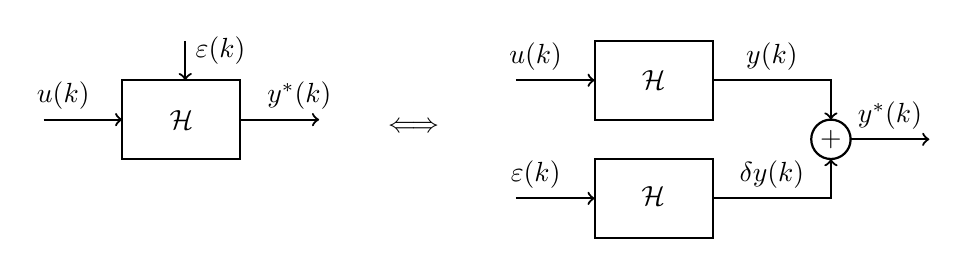
\begin{tikzpicture}[x=1cm,y=1cm]
				\draw (-9, 0.5) -- (-8,0.5) [->, thick] node[above,near start]{$\boldsymbol{u}(k)$};
				\draw (-7.2, 1.5) -- (-7.2,1.0) [->, thick] node[right,near start]{$\boldsymbol{\varepsilon}(k)$};
				\draw (-6.5, 0.5) -- (-5.5,0.5) [->, thick] node[above,near end]{$\boldsymbol{y}^*(k)$};
				\draw (-8,0.0) rectangle ++(1.5,1)[thick] node [midway]{$\mathcal{H}$}; 
				\draw (-2,0.5) rectangle ++(1.5,1)[thick] node [midway]{$\mathcal{H}$}; 
				\draw (-3, 1) -- (-2,1) [->, thick] node [above,near start]{$\boldsymbol{u}(k)$}; 
				\draw (-0.5, 1)  -- (1,1) -- (1,0.5) [->, thick] node[xshift=-0.75cm,yshift=0.8cm]{$\boldsymbol{y}(k)$}; 

				\draw (-2,-1) rectangle ++(1.5,1)[thick] node [midway]{$\mathcal{H}_{\abserr}$}; 
				\draw (-3, -0.5) -- (-2,-0.5) [->, thick] node[above,near start]{$\boldsymbol{\varepsilon}(k)$};
				\draw (-0.5, -0.5) -- (1,-0.5) -- (1,0) [->, thick] node [xshift=-0.75cm,yshift=-0.2cm]{$\boldsymbol{\delta y}(k)$}; 

				\draw (1,0.25) circle (0.25) [thick] node {$+$}; 
				\draw (1.25,0.25) -- (2.25,0.25)[->, thick] node [above,midway] {$\boldsymbol{y}^*(k)$};

				\node (arrow) at (-4.3,0.4) {$\iff$};
			  \end{tikzpicture}

			\caption{A signal view of the error propagation with respect to the ideal filter \label{fig:ltierror}}
			\end{figure}


		According to \ref{zmatrix}, we have:

		\begin{equation} \label{zepsmatrix}
		\boldsymbol{Z_\varepsilon}=
					\begin{pmatrix}
						\boldsymbol{-J} & \boldsymbol{M} & \boldsymbol{M}_t \\
						\boldsymbol{K} & \boldsymbol{P} & \boldsymbol{M}_x \\
						\boldsymbol{L} & \boldsymbol{R} & \boldsymbol{M}_y 
					\end{pmatrix}
		\end{equation}

		with:
		\begin{eqnarray} \label{deltaerr}
			\boldsymbol{M}_t=(\boldsymbol{I}_{n_t} \boldsymbol{0}_{n_t \times n_x} \boldsymbol{0}_{n_t \times n_y}), \\
			\boldsymbol{M}_x=(\boldsymbol{0}_{n_x \times n_x} \boldsymbol{I}_{n_x} \boldsymbol{0}_{n_x \times n_y}), \\
			\boldsymbol{M}_y=(\boldsymbol{0}_{n_y \times n_t} \boldsymbol{0}_{n_y \times n_x} \boldsymbol{I}_{n_y}),
		\end{eqnarray}

		$\mathcal{H}_{\boldsymbol{\varepsilon}}$ is a filter with ($n_t+n_x+n_u$) inputs and $n_y$ outputs.
		\begin{proposition}
			The transfert function of filter $\mathcal{H_{\boldsymbol{\varepsilon}}}$, denoted $\boldsymbol{H}_\varepsilon$, is defined as follows:
			\begin{equation}
				\boldsymbol{H}_{\varepsilon}: \rightarrow \boldsymbol{C_Z}(z\boldsymbol{I}_n-\boldsymbol{A_Z})^{-1}\boldsymbol{M}_1 +\boldsymbol{M}_2 \hspace{5pt} \forall z \in \mathbb{C}
			\end{equation}
			with $\boldsymbol{A_Z}$ and $\boldsymbol{C_Z}$ the matrices defined by \ref{abcdtranspose} and
			\begin{equation}
				\boldsymbol{M_1}=(\boldsymbol{KJ}^{-1}   \hspace{10pt}\boldsymbol{I}_{n_x} \hspace{10pt} \boldsymbol{0}), \hspace{5pt}
				\boldsymbol{M_2}=(\boldsymbol{LJ}^{-1}  \hspace{10pt}\boldsymbol{0} \hspace{10pt}\boldsymbol{I}_{n_y}), 
			\end{equation}
		\end{proposition}
		The demonstration is well detailed in Lopez' PhD \cite{lopez}.

		\begin{corollary} \label{corimp}
			Considering a filter $\mathcal{H}$, $\boldsymbol{\varepsilon}(k)$ the vector of computation errors at time k in the finite precision of $\mathcal{H}$,
			and $\mathcal{H}\boldsymbol{\varepsilon}$ the error filter associated to $\mathcal{H}$.
			The behaviour of error can be described from $\boldsymbol{\varepsilon}(k)$ and $\mathcal{H}\boldsymbol{\varepsilon}$.
			We consider the error as an interval vector, denoted by its center and radius $\langle \boldsymbol{\varepsilon}_m, \boldsymbol{\varepsilon}_r \rangle$ and 
			the interval vector of global error $\boldsymbol{\delta y}$, denoted $\langle \boldsymbol{\delta y}_m, \boldsymbol{\delta y}_r \rangle$.
			In practise, all inputs are centered around zero, which is not the case in the command community, where this notation makes sense.
			So we consider that $\boldsymbol{\varepsilon}_m=0$.
			The results are the following:

			\begin{eqnarray} \label{eqprec}
				\boldsymbol{\delta y}_m = 0 \\
				\boldsymbol{\delta y}_r = \langle\langle \mathcal{H}_{\boldsymbol{\varepsilon}} \rangle\rangle_{wcpg} \cdot \boldsymbol{\varepsilon}_r
			\end{eqnarray}
		\end{corollary}

		In the future we will then get rid of $boldsymbol{\delta y}_m$.

		Let's define:
			$$n'=n_t+n_x+n_y$$

		and:

			\begin{equation}
				\boldsymbol{v'}=
				\begin{pmatrix}
					\boldsymbol{t}(k+1) \\
					\boldsymbol{x}(k+1) \\
					\boldsymbol{y}(k)   \\
				\end{pmatrix}
			\end{equation}


		Then, following Lopez's computations, we can derive precisions for every intermediate step:
		
		\begin{equation}
			|\boldsymbol{\delta y}_i| \leq \sum_{j=1}^{n'} | \langle\langle \mathcal{H}_{\boldsymbol{\varepsilon}} \rangle\rangle_{i,j}| \cdot \boldsymbol{2^{l_{v'_j}}}
		\end{equation}

		To formalize with a matricial formulation, we get:
		\begin{equation}
			|\boldsymbol{\delta y}| \leq | \langle\langle \mathcal{H}_{\boldsymbol{\varepsilon}} \rangle\rangle| \cdot \boldsymbol{2^{lsb_{v'}}}
		\end{equation}


		To satisfy the condition \ref{condition}, we can simply define $\xi$ as the minimal error the user wants.
		We can then state:
		\begin{equation}
			| \langle\langle \mathcal{H}_{\boldsymbol{\varepsilon}} \rangle\rangle| \cdot \boldsymbol{2^{lsb_{v'}}} < \xi
		\end{equation}

		That is, 
		\begin{equation} \label{constraint}
			\boldsymbol{\mathfrak{A}} \cdot \boldsymbol{2}^{lsb_{v'}-msb_{v'}-1} < \boldsymbol{1}_{n_y}
			%\boldsymbol{D} \cdot \boldsymbol{2}^{lsb_{v'}-msb_{v'}-1} < \boldsymbol{1}_{n_y}
		\end{equation}

		Where:
		\begin{eqnarray}
			\boldsymbol{\mathfrak{A}}_{i,j}= | \langle\langle \mathcal{H}_{\boldsymbol{\varepsilon}} \rangle\rangle_{i,j} | \cdot \frac{\boldsymbol{2^{msb_{v'_j}+1}}}{\xi_i} %\\
			%\boldsymbol{D}_{i,j}= | \langle\langle \mathcal{H}_{\boldsymbol{\varepsilon}} \rangle\rangle_{i,j}| \cdot \frac{\boldsymbol{2^{msb_{v'_j}+1}}}{\xi_i}
		\end{eqnarray}

		So, for computations in arbitrary precision, we have here a sufficient condition (\ref{constraint}) to implement the filters.

		%\TODO: check if this step is sufficient.

%		\subsubsection{A working solution to this problem}
%		A solution poposed in Lopez's PhD \cite{lopez}, is to consider the following reformulation of constraint \ref{constraint}.
%		We can give a stronger majoration, as follows:
%		\begin{equation}
%			\frac{\mathfrak{A}_{i1}}{\boldsymbol{2}^{msb_{v'_1}-lsb_{v'_1}+1}} + \frac{\mathfrak{A}_{i2}}{\boldsymbol{2}^{msb_{v'_2}-lsb_{v'_2}+1}} + \dots + \frac{\mathfrak{A}_{in'}}{\boldsymbol{2}^{msb_{v'_{n'}}-lsb_{v'_{n'}}+1}} < 1, \hspace{5pt} \forall 1 \leq i \leq n_y 
%		\end{equation}
		
		\subsubsection{Worst-case peak gain computation}
			Computing the worst-case peak gain accurately in finite precision is a very complex problem.
			As we can't afford doing such a work, we are about to integrate code developped by Anastasia Lozanova Volkova from Hilaire's team at LIP6 \cite{Volk15a}, under the metalibm project.










%	\subsection{Adjustments in arbitrary precision}

	





%		
%	\subsection{Canonical specification}
%		
%		The intuitive and first way to describe an LTI filter is to specify the output as a function of the inputs:
%		$$y(k)=\sum_{i=0}^n b_i u(k-i)-\sum_{i=1}^n a_i y(k-i)$$
%
%	\subsection{Z transform}
%	$$X(z)=\mathcal{Z}\{x\}=\sum_{k=0}^{+\infty} x(k) z^{-k}$$
%	
%	\subsection{Transfert Function}
%	A filter is usually described by it's transfert function, defined as:
%
%	$$H(z)=\frac{Y(z)}{U(z)}=\frac{\sum_{i=0}^n b_i z^{-i}}{ 1 + \sum_{i=1}^n a_i z^{-i}}, \;\;\;\; \forall z \in \mathbb{C}$$ 
%	\subsection{Impulse response}
%	$\delta$
%	\subsection{Worst case peak gain (WCPG)}
%	$$\| \mathcal{H} \|_{WCPG}=\sup_{i\neq 0} \frac{\|h*u\|_{l^\infty}}{\|u\|_{l^\infty}} $$
%
%	$$\| \mathcal{H} \|_{WCPG}= \sum_{k \geq 0} |h(k)| $$
%	\subsection{Realisations}



	



